\chapter{Distribución de Laplace}

En estadística y en teoría de la probabilidad la distribución de Laplace es una densidad de probabilidad continua, llamada así en honor a Pierre-Simon Laplace. Es también conocida como distribución doble exponencial puesto que puede ser considerada como la relación las densidades de dos distribuciones exponenciales adyacentes. \cite{wiki:5}

\section{Descripción}

Se utiliza la distribución de Laplace cuando la distribución de los datos tenga un pico más alto que una distribución normal.Por ejemplo, la distribución de Laplace se utiliza para modelar en biología, finanzas y economía.

\section{PDF}
\begin{center}
	$\frac {1}{2,b} \exp(-\frac {|x-\mu|}{b})$
\end{center}
\subsection{Parámetros}
Los parámetros observables son:

\begin{center}
	\begin{tabular} {| l | l |}
		\hline
		$\mu$ & Parámetro de localización \\ \hline
		b & Parámetro de escala\\ \hline
	\end{tabular}
\end{center}

\section{CDF}
\begin{center}
	$\frac {1}{2} \exp(\frac {x-\mu}{b})$
\end{center}

\section{MGF}
\begin{center}
	$\frac{\exp(\mu \,t)}{1-b^{2}\,t^{2}}$
\end{center}

\section{Media y Varianza}
\subsection{Media}
\begin{center}
	$\mu$
\end{center}

\subsection{Varianza}
\begin{center}
	$2b^2$
\end{center}
	
\section{Gráficas}
\begin{center}
	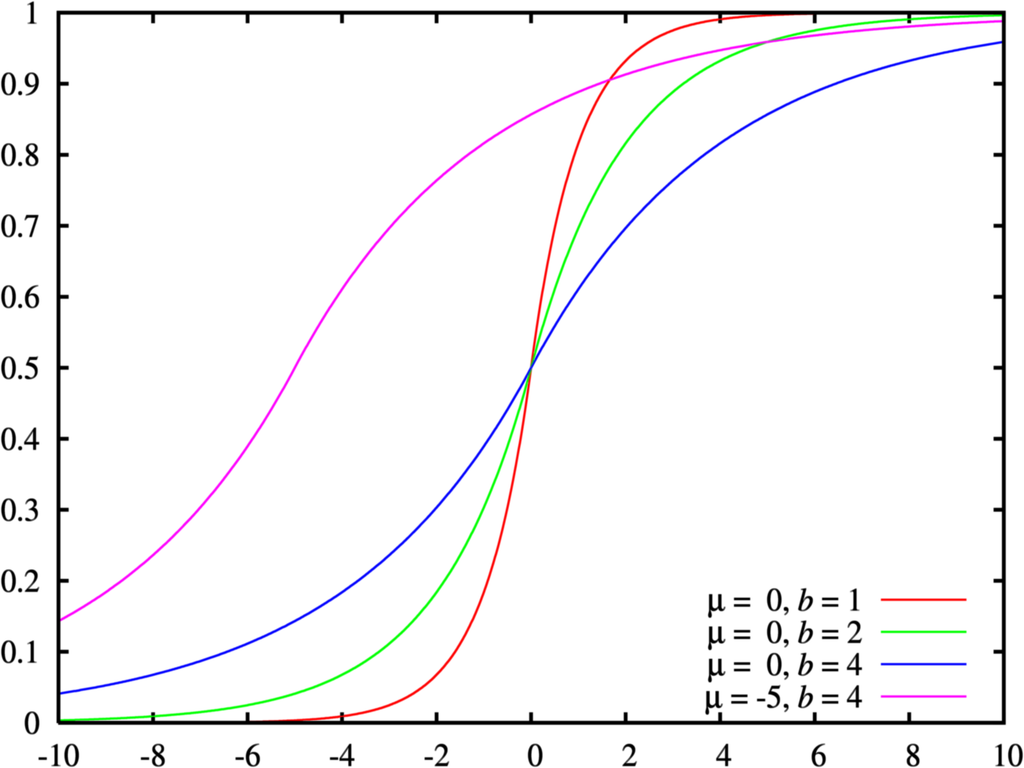
\includegraphics[scale=0.3]{imgs/laplace-cdf.png}
	
	\textit{CDF}
\end{center}

\begin{center}
	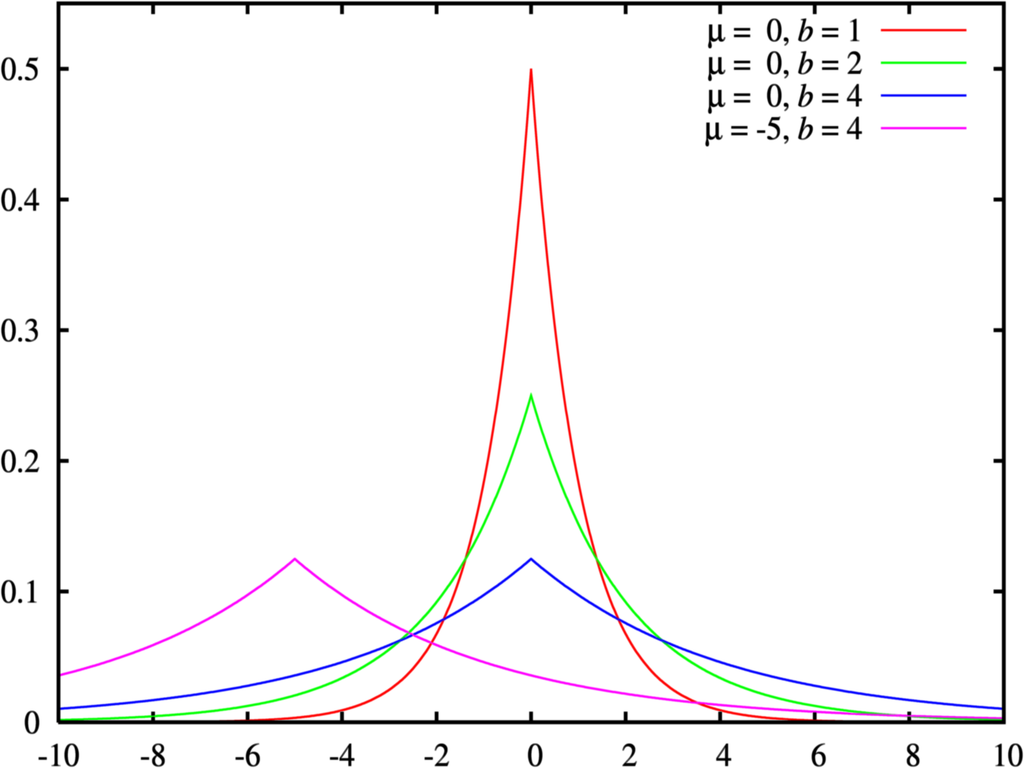
\includegraphics[scale=0.3]{imgs/laplace-pdf.png}
	
	\textit{PDF}
\end{center}
	
\section{Aplicaciones en la vida real}
La distribución laplaciana se ha utilizado en el reconocimiento de voz y en la compresión de imágenes JPEG.